%++++++++++++++++++++++++++++++++++++++++s\\
\documentclass[letterpaper,12pt]{article}
\usepackage{tabularx} % extra features for tabular environment
\usepackage{amsmath}  % improve math presentation
\usepackage{graphicx} % takes care of graphic including machinery
\usepackage[margin=1in,letterpaper]{geometry} % decreases margins
\usepackage{cite} % takes care of citations
\usepackage[final]{hyperref} % adds hyper links inside the generated pdf file
\usepackage{caption}
\usepackage{float}
\usepackage{subcaption}
\hypersetup{
	colorlinks=true,       % false: boxed links; true: colored links
	linkcolor=blue,        % color of internal links
	citecolor=blue,        % color of links to bibliography
	filecolor=magenta,     % color of file links
	urlcolor=blue         
}
%++++++++++++++++++++++++++++++++++++++++


\begin{document}

\title{732A75 Advanced Data Mining laboratory 1 report}
\author{Yuki Washio and Nicolas Taba}
\date{\today}
\maketitle



\section{Introduction}

The aim of this laboratory exercise is to gain familiarity with the data mining toolkit Weka by using some of its clustering algorithms and analyzing their output.

In this laboratory, we use the HARTIGAN (file06) dataset. This dataset features 27 kinds of food and informs us of the energy, protein, fat,c alcium and iron content per 3 ounce of portion.


\section{Clustering using the Kmeans algorithm}

In this section of the laboratory, we use the Kmeans algortithm to cluster the data. We choose to ignore the "name" label because the algortihm does not interpret names as words but as strings. The Kmeans algorithm would try to measure distances between strings which is not a good metric. However, we notice that all of the food are meat and seafood based.

We experiment with the clustering algorithm by trying 2 different number of cluster (2 and 5) starting with the same initial cluster center (seed 10).

\subsection{2 clusters with seed 10}



The clustering algorithm separates into two clusters with 9 and 18 elements respectively in each Fig.~\ref{fig:kmeans_10_2_out}. We observe a linear relationship between fat as a function of energy Fig.~\ref{fig:sub-first_1}. We seem to be able to separate the clusters into High energy, high fat the second cluster having low values for those labels. The clusters seem to be made up of similar elements that discriminate mostly along the energy values as we can see in the graphs that depict Protein, calcium and iron as a function of energy respectively.

\begin{figure}[H] 
  \centering
      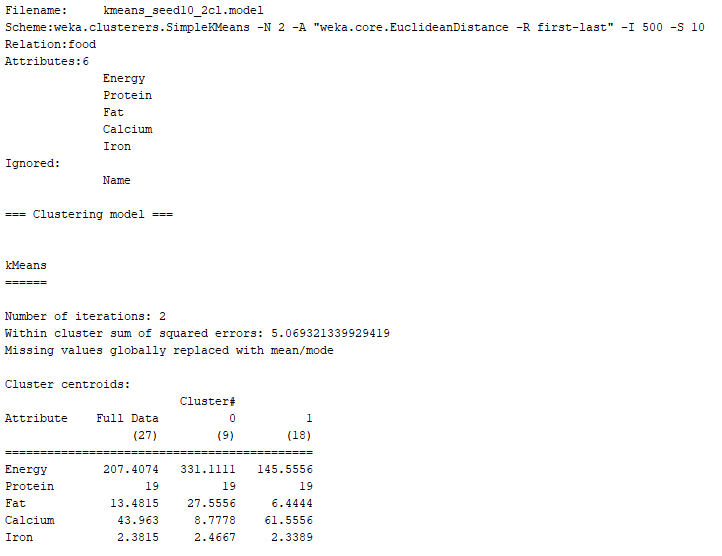
\includegraphics[width=0.5\columnwidth]{kmeans_seed10_2cl_output}

% copy paste this template for figures/images.
% will check how to add multiple images one next another
        \caption{
                \label{fig:kmeans_10_2_out}  
                Kmeans algorithm output from Weka for 2 clusters, using seed 10.
        }
\end{figure}

\begin{figure}[H]
\begin{subfigure}{.4\textwidth}
  \centering
  % include first image
  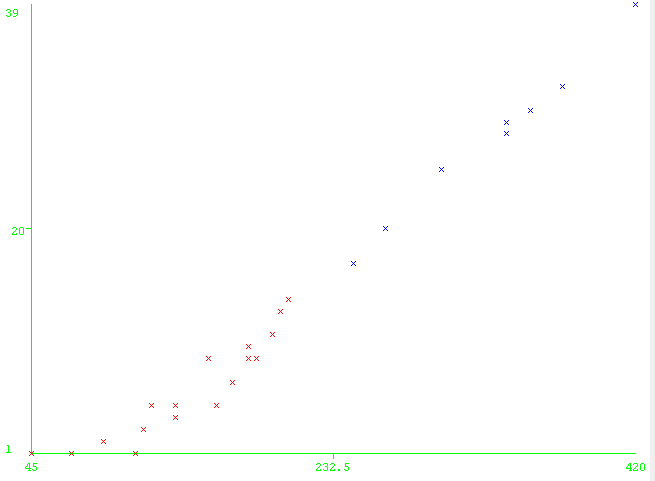
\includegraphics[width=.8\linewidth]{kmeans_seed10_2cl_energy_fat}  
  \caption{fat as a function of energy}
  \label{fig:sub-first_1}
\end{subfigure}
\begin{subfigure}{.4\textwidth}
  \centering
  % include second image
  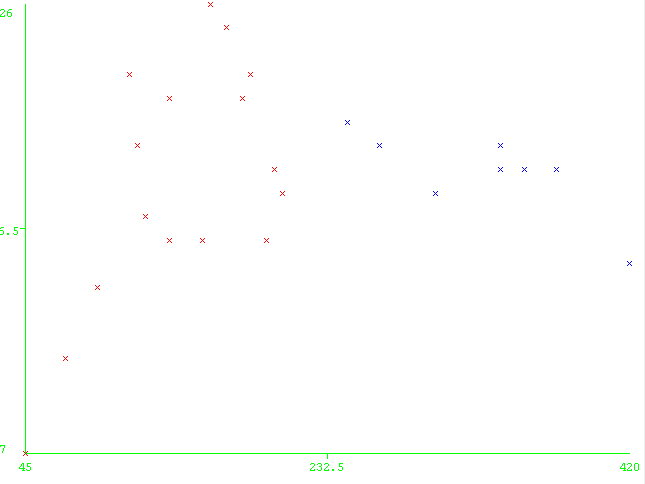
\includegraphics[width=.8\linewidth]{kmeans_seed10_2cl_energy_protein}  
  \caption{protein as a function of energy}
  \label{fig:sub-second_1}
\end{subfigure}

%\newline

\begin{subfigure}{.4\textwidth}
  \centering
  % include third image
  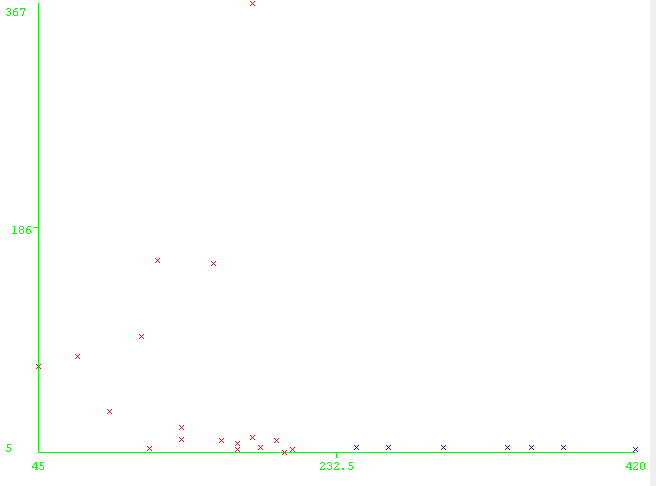
\includegraphics[width=.8\linewidth]{kmeans_seed10_2cl_energy_calcium}  
  \caption{Calcium as a function of energy}
  \label{fig:sub-third_1}
\end{subfigure}
\begin{subfigure}{.4\textwidth}
  \centering
  % include third image
  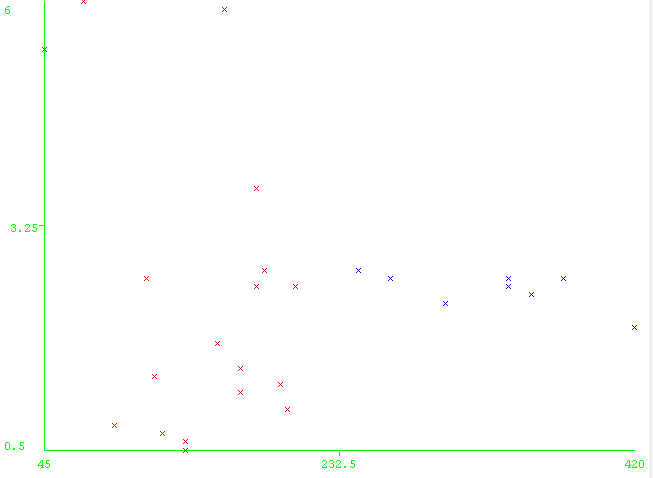
\includegraphics[width=.8\linewidth]{kmeans_seed10_2cl_energy_iron}  
  \caption{Iron as a function of energy}
  \label{fig:sub-fourth_1}
\end{subfigure}
\caption{Cluster plot for Kmeans for 2 clusters}
\label{fig:fig_1}
\end{figure}

It is difficult to assign proper names to these clusters from the data shown in the cluster plots. However, we know that the data itself is of seafood and meats and we observed a linear relationship between the fat and energy parameters. We know that red meats contain more fat than seafood. One would push forwar that we could separate cluster-wise according to this principle. Further investigation of the dataset is needed.


\subsection{5 clusters with seed 10}

The clusters include all the points, but some of the elements of the same clusters are very dissimilar. In Fig.~\ref{fig:sub-fourth_3} we can see that the elements of the green cluster are dissimilar to each other when observing iron with respect to energy. This intra-cluster dissimilarity is observed for other variables. These are bad clusters as they have high dissimilarity between elements compared to the previous solution with 2 clusters. We can conclude that one must be careful when choosing the appropriate number of clusters in order for this algorithm to work. 

A special attention should be given to the type of data that is being analyzed. As noted previously, we know from the name of the data that it can be separated by red meats and seafood. There might be other ways of separating the data differently, but it is not immediately evident what 5 clusters could be made from the data.

\begin{figure}[H] 
  \centering
      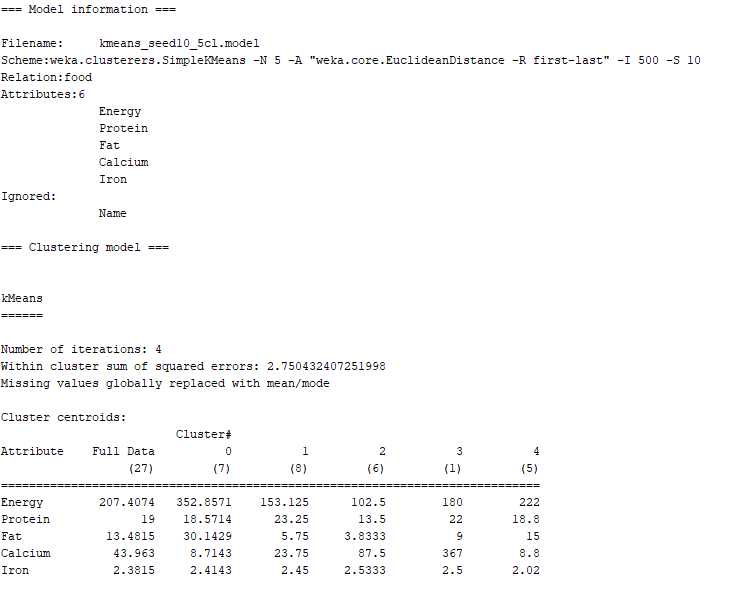
\includegraphics[width=0.5\columnwidth]{kmeans_seed10_5cl_output}

% copy paste this template for figures/images.
% will check how to add multiple images one next another
        \caption{
                \label{fig:kmeans_10_5_out}  
                Kmeans algorithm output from Weka for 5 clusters, using seed 10.
        }
\end{figure}


\begin{figure}[H]
\begin{subfigure}{.4\textwidth}
  \centering
  % include first image
  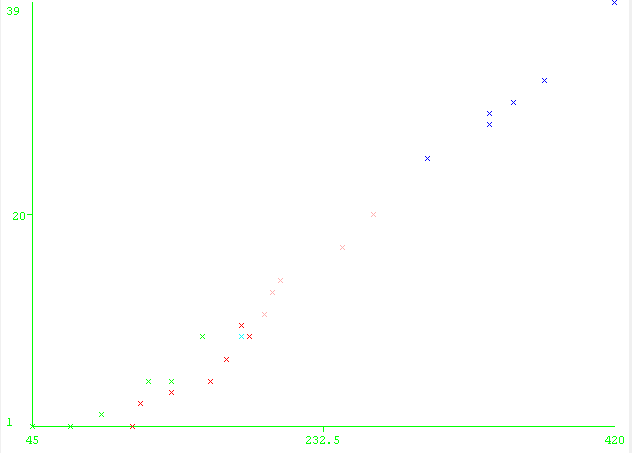
\includegraphics[width=.8\linewidth]{kmeans_seed10_5cl_energy_fat}  
  \caption{fat as a function of energy}
  \label{fig:sub-first_3}
\end{subfigure}
\begin{subfigure}{.4\textwidth}
  \centering
  % include second image
  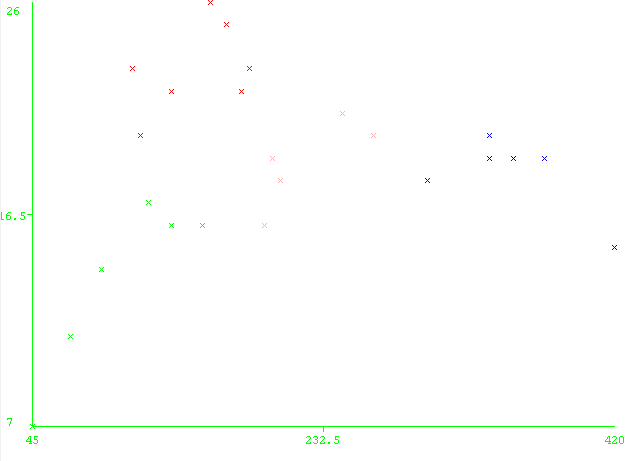
\includegraphics[width=.8\linewidth]{kmeans_seed10_5cl_energy_protein}  
  \caption{protein as a function of energy}
  \label{fig:sub-second_3}
\end{subfigure}

%\newline

\begin{subfigure}{.4\textwidth}
  \centering
  % include third image
  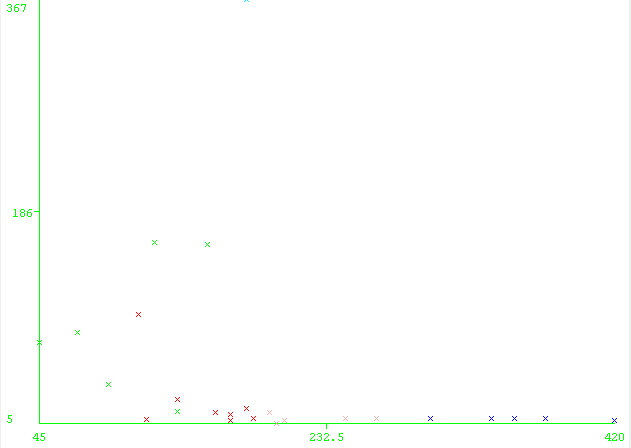
\includegraphics[width=.8\linewidth]{kmeans_seed10_5cl_energy_calcium}  
  \caption{Calcium as a function of energy}
  \label{fig:sub-third_3}
\end{subfigure}
\begin{subfigure}{.4\textwidth}
  \centering
  % include third image
  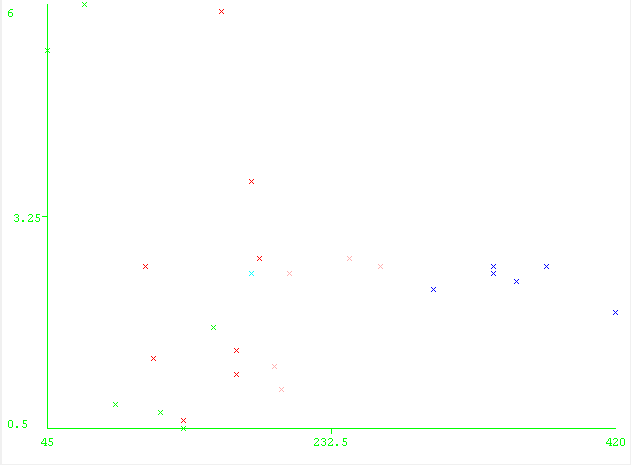
\includegraphics[width=.8\linewidth]{kmeans_seed10_5cl_energy_iron}  
  \caption{Iron as a function of energy}
  \label{fig:sub-fourth_3}
\end{subfigure}
\caption{Cluster plot for Kmeans with 5 clusters}
\label{fig:fig_3}
\end{figure}



\subsection{2 clusters with seed 1 and 123}

We observe poor clustering when using seed 123, the elements within the clusters are dissimilar to one another as seen in Fig.~\ref{fig:sub-third_2} as attested by the larger sum of square error compared to the two other clustering solutions. We also notice that there are only two element in cluster 0.

When using different seed, we obtain similar, plausible results. For example, seed 1 yields similar results than those obtained for seed 10. This reinforces our belief that the clustering algorithms yields the correct result given that the other parameters are fixed (number of clusters and data). Our conclusion that the food be separated into 2 categories is reinforced, however it becomes more difficult to decide which one of these clustering solutions is the correct one. The metric we choose to separate the better clustering is the sum of square error in this case. We will choose seed 10.

The seed value controls the generation of random numbers. This in turn decides where the starting centroid is chosen to be in the algorithm. Different seed number will yield different clusters. The seed is intended to be used for reproducibility of results by different users.

% This is how you add several pictures to the same larger "figure"
\begin{figure}[H]
\begin{subfigure}{.4\textwidth}
  \centering
  % include first image
  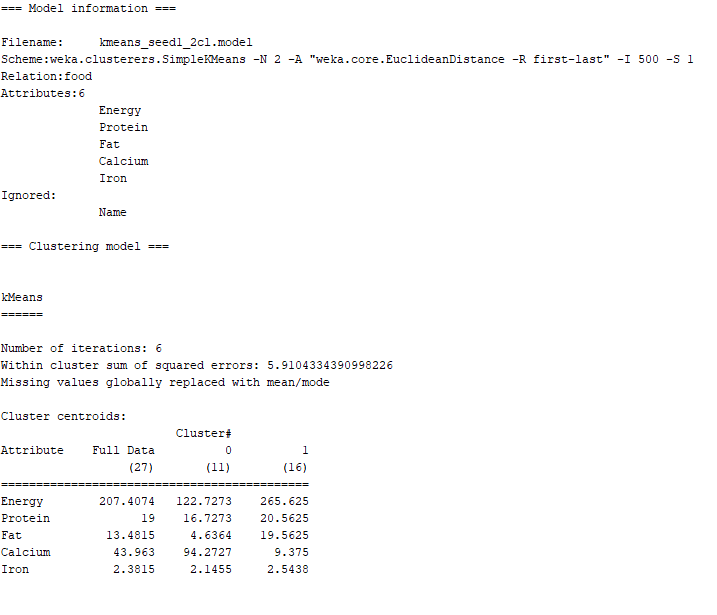
\includegraphics[width=.8\linewidth]{kmeans_seed1_2cl_output}  
  \caption{Kmeans using seed 1}
  \label{fig:sub-first_2}
\end{subfigure}
\begin{subfigure}{.4\textwidth}
  \centering
  % include second image
  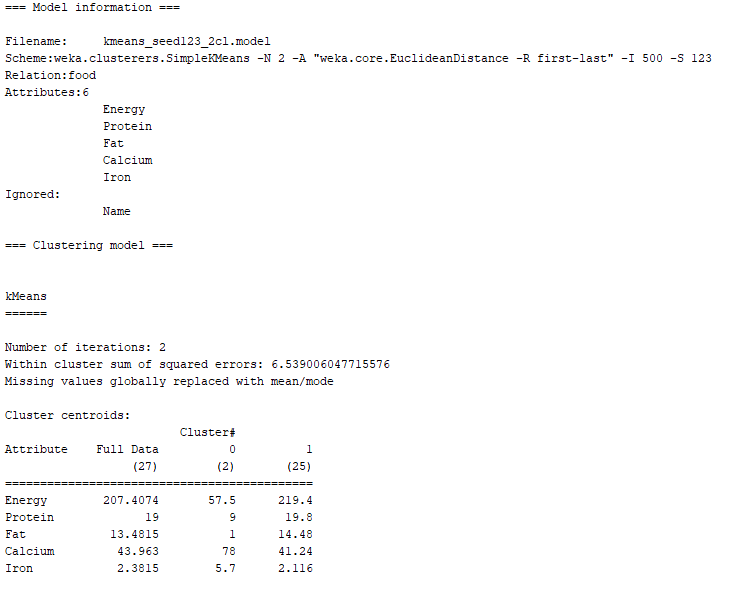
\includegraphics[width=.8\linewidth]{kmeans_seed123_2cl_output}  
  \caption{Kmeans using seed 123}
  \label{fig:sub-second_2}
\end{subfigure}

%\newline

\begin{subfigure}{.4\textwidth}
  \centering
  % include third image
  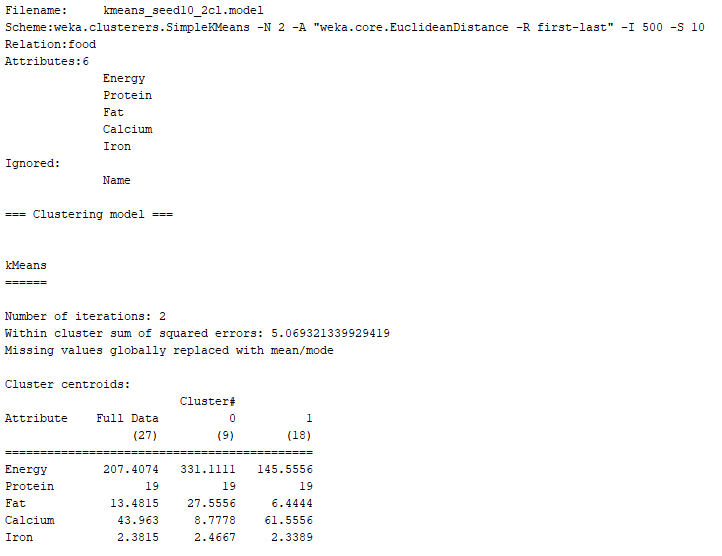
\includegraphics[width=.8\linewidth]{kmeans_seed10_2cl_output}  
  \caption{Kmeans using seed 10}
  \label{fig:sub-third_2}
\end{subfigure}
\caption{Kmeans algorithm for 2 clusters using different seed}
\label{fig:fig_2}
\end{figure}




\section{Using density based clusters}

We use here density based clusters to cluster our data. This approach allows us to control how large we allow clusters to vary from their centroid by tuning the standard deviation parameter. We use the SimpleKMeans clusterer with $k = 2$ and seed 10. We will change use values of the standard deviation of $1.e^{-6}$ and $200$.

We start with the density based clustering that uses the smallest standard deviation first.




\begin{figure}[H]
\begin{subfigure}{.4\textwidth}
  \centering
  % include first image
  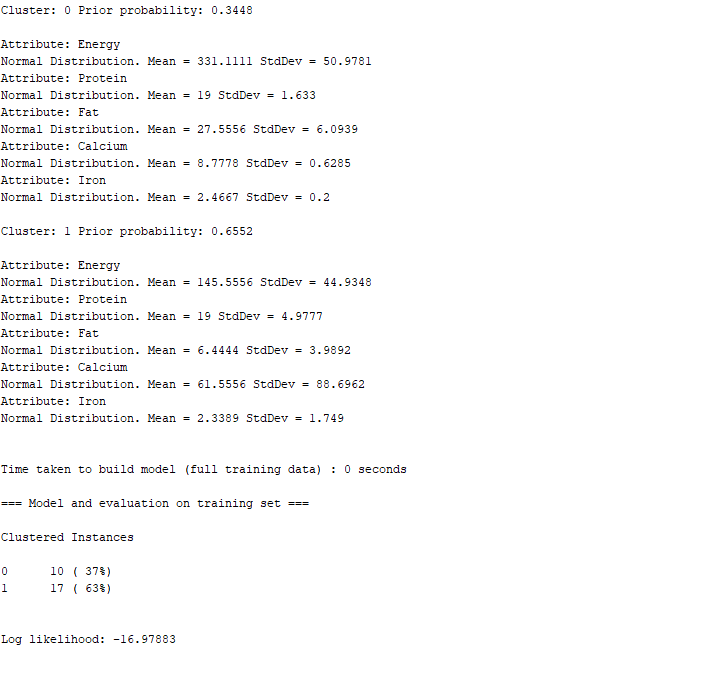
\includegraphics[width=.8\linewidth]{density_seed10_cl2_devE-6}  
  \caption{Density based clustering output}
  \label{fig:sub-first_4}
\end{subfigure}
\begin{subfigure}{.4\textwidth}
  \centering
  % include second image
  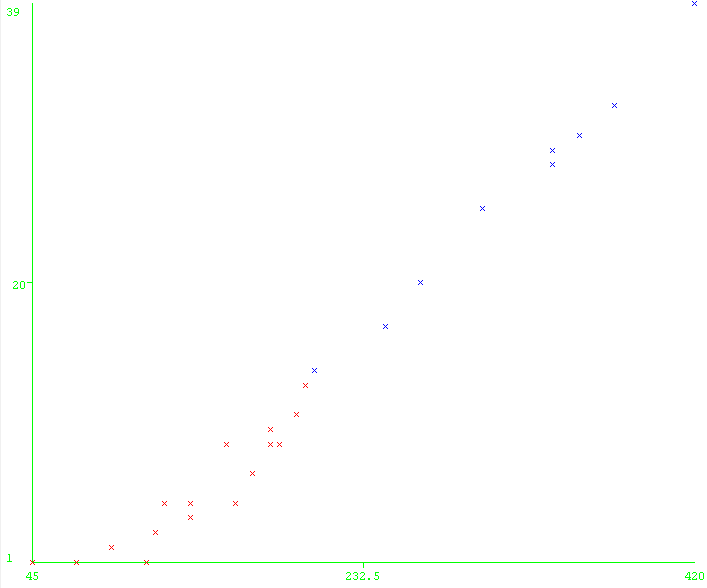
\includegraphics[width=.8\linewidth]{density_e6_energy_fat}  
  \caption{Cluster plot of energy with respect to fat}
  \label{fig:sub-second_4}
\end{subfigure}
\caption{Density based clustering with standard deviation of $1.e^{-6}$}
\label{fig:fig_4}
\end{figure}



We obtain similar results to the ones we previously had using the kmeans approach. Furthermore, we can observe that the clustering by visualizing fat with respect to energy in Fig.~\ref{fig:sub-second_4} is similar to that obtained previously in Fig.~\ref{fig:sub-first_1}


We now increase the standard deviation to 200 while keeping all other arguments the same.

\begin{figure}[H]
\begin{subfigure}{.4\textwidth}
  \centering
  % include first image
  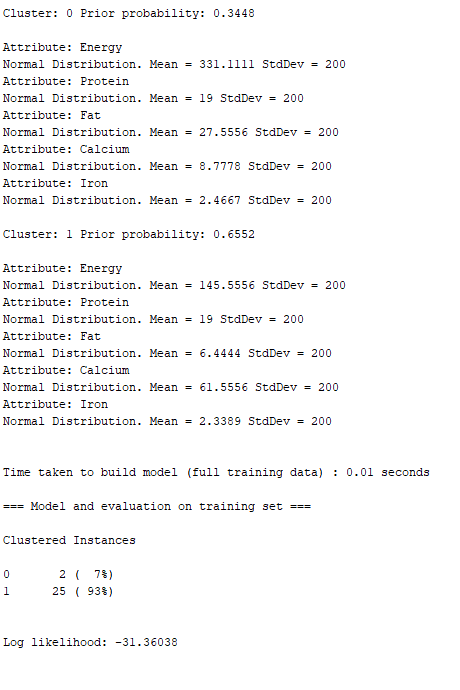
\includegraphics[width=.8\linewidth]{density_seed10_cl2_dev200}  
  \caption{Density based clustering output}
  \label{fig:sub-first_4}
\end{subfigure}
\begin{subfigure}{.4\textwidth}
  \centering
  % include second image
  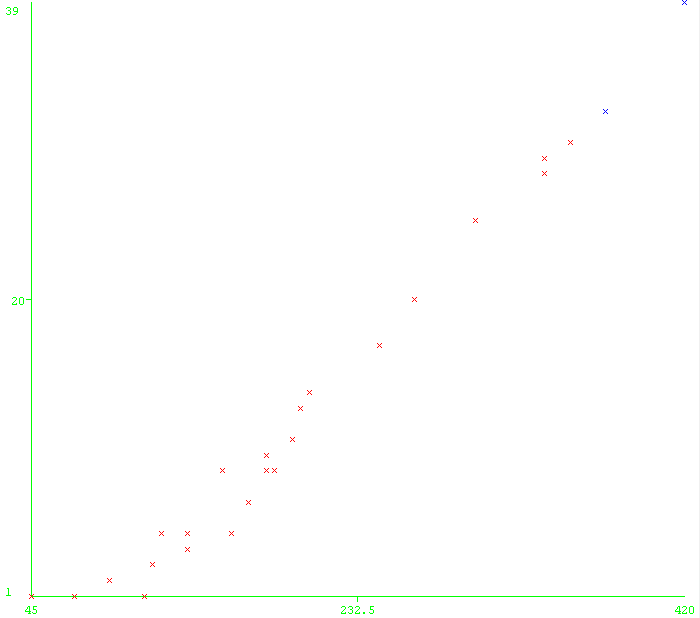
\includegraphics[width=.8\linewidth]{density_200_energy_fat}  
  \caption{Cluster plot of energy with respect to fat}
  \label{fig:sub-second_4}
\end{subfigure}
\caption{Density based clustering with standard deviation of 200}
\label{fig:fig_5}
\end{figure}


We observe from the data in Fig.~\ref{fig:fig_5} that the when the standard deviation is large enough, we have clusters with large dissimilarity returned to us by the algorithm. As pointed out earlier, a high standard deviation parameter will result in large amounts of data that are dissimilar to the centroid to be accepted as part of the cluster. This is due to the fact that with  a high enough standard deviation, the density for elements that are far from the centroid is high enough to be accepted in the first cluster that is calculated.

In conclusion, we should pay attention to the value we assign to standard deviation as a value that is too high will yield poor quality clusters with dissimilar items within them.

\end{document}
